% Options for packages loaded elsewhere
\PassOptionsToPackage{unicode}{hyperref}
\PassOptionsToPackage{hyphens}{url}
\PassOptionsToPackage{dvipsnames,svgnames,x11names}{xcolor}
%
\documentclass[
  twocolumn,
  landscape]{report}

\usepackage{amsmath,amssymb}
\usepackage{iftex}
\ifPDFTeX
  \usepackage[T1]{fontenc}
  \usepackage[utf8]{inputenc}
  \usepackage{textcomp} % provide euro and other symbols
\else % if luatex or xetex
  \usepackage{unicode-math}
  \defaultfontfeatures{Scale=MatchLowercase}
  \defaultfontfeatures[\rmfamily]{Ligatures=TeX,Scale=1}
\fi
\usepackage[]{libertinus}
\ifPDFTeX\else  
    % xetex/luatex font selection
\fi
% Use upquote if available, for straight quotes in verbatim environments
\IfFileExists{upquote.sty}{\usepackage{upquote}}{}
\IfFileExists{microtype.sty}{% use microtype if available
  \usepackage[]{microtype}
  \UseMicrotypeSet[protrusion]{basicmath} % disable protrusion for tt fonts
}{}
\makeatletter
\@ifundefined{KOMAClassName}{% if non-KOMA class
  \IfFileExists{parskip.sty}{%
    \usepackage{parskip}
  }{% else
    \setlength{\parindent}{0pt}
    \setlength{\parskip}{6pt plus 2pt minus 1pt}}
}{% if KOMA class
  \KOMAoptions{parskip=half}}
\makeatother
\usepackage{xcolor}
\usepackage[top=30mm,left=20mm,heightrounded]{geometry}
\setlength{\emergencystretch}{3em} % prevent overfull lines
\setcounter{secnumdepth}{-\maxdimen} % remove section numbering
% Make \paragraph and \subparagraph free-standing
\ifx\paragraph\undefined\else
  \let\oldparagraph\paragraph
  \renewcommand{\paragraph}[1]{\oldparagraph{#1}\mbox{}}
\fi
\ifx\subparagraph\undefined\else
  \let\oldsubparagraph\subparagraph
  \renewcommand{\subparagraph}[1]{\oldsubparagraph{#1}\mbox{}}
\fi


\providecommand{\tightlist}{%
  \setlength{\itemsep}{0pt}\setlength{\parskip}{0pt}}\usepackage{longtable,booktabs,array}
\usepackage{calc} % for calculating minipage widths
% Correct order of tables after \paragraph or \subparagraph
\usepackage{etoolbox}
\makeatletter
\patchcmd\longtable{\par}{\if@noskipsec\mbox{}\fi\par}{}{}
\makeatother
% Allow footnotes in longtable head/foot
\IfFileExists{footnotehyper.sty}{\usepackage{footnotehyper}}{\usepackage{footnote}}
\makesavenoteenv{longtable}
\usepackage{graphicx}
\makeatletter
\def\maxwidth{\ifdim\Gin@nat@width>\linewidth\linewidth\else\Gin@nat@width\fi}
\def\maxheight{\ifdim\Gin@nat@height>\textheight\textheight\else\Gin@nat@height\fi}
\makeatother
% Scale images if necessary, so that they will not overflow the page
% margins by default, and it is still possible to overwrite the defaults
% using explicit options in \includegraphics[width, height, ...]{}
\setkeys{Gin}{width=\maxwidth,height=\maxheight,keepaspectratio}
% Set default figure placement to htbp
\makeatletter
\def\fps@figure{htbp}
\makeatother

\makeatletter
\makeatother
\makeatletter
\makeatother
\makeatletter
\@ifpackageloaded{caption}{}{\usepackage{caption}}
\AtBeginDocument{%
\ifdefined\contentsname
  \renewcommand*\contentsname{Table of contents}
\else
  \newcommand\contentsname{Table of contents}
\fi
\ifdefined\listfigurename
  \renewcommand*\listfigurename{List of Figures}
\else
  \newcommand\listfigurename{List of Figures}
\fi
\ifdefined\listtablename
  \renewcommand*\listtablename{List of Tables}
\else
  \newcommand\listtablename{List of Tables}
\fi
\ifdefined\figurename
  \renewcommand*\figurename{Figure}
\else
  \newcommand\figurename{Figure}
\fi
\ifdefined\tablename
  \renewcommand*\tablename{Table}
\else
  \newcommand\tablename{Table}
\fi
}
\@ifpackageloaded{float}{}{\usepackage{float}}
\floatstyle{ruled}
\@ifundefined{c@chapter}{\newfloat{codelisting}{h}{lop}}{\newfloat{codelisting}{h}{lop}[chapter]}
\floatname{codelisting}{Listing}
\newcommand*\listoflistings{\listof{codelisting}{List of Listings}}
\makeatother
\makeatletter
\@ifpackageloaded{caption}{}{\usepackage{caption}}
\@ifpackageloaded{subcaption}{}{\usepackage{subcaption}}
\makeatother
\makeatletter
\@ifpackageloaded{tcolorbox}{}{\usepackage[skins,breakable]{tcolorbox}}
\makeatother
\makeatletter
\@ifundefined{shadecolor}{\definecolor{shadecolor}{rgb}{.97, .97, .97}}
\makeatother
\makeatletter
\makeatother
\makeatletter
\makeatother
\ifLuaTeX
  \usepackage{selnolig}  % disable illegal ligatures
\fi
\IfFileExists{bookmark.sty}{\usepackage{bookmark}}{\usepackage{hyperref}}
\IfFileExists{xurl.sty}{\usepackage{xurl}}{} % add URL line breaks if available
\urlstyle{same} % disable monospaced font for URLs
\hypersetup{
  pdftitle={Thermodynamics paper},
  colorlinks=true,
  linkcolor={blue},
  filecolor={Maroon},
  citecolor={Blue},
  urlcolor={Blue},
  pdfcreator={LaTeX via pandoc}}

\title{Thermodynamics paper}
\author{}
\date{}

\begin{document}
\maketitle
\ifdefined\Shaded\renewenvironment{Shaded}{\begin{tcolorbox}[boxrule=0pt, frame hidden, interior hidden, borderline west={3pt}{0pt}{shadecolor}, sharp corners, enhanced, breakable]}{\end{tcolorbox}}\fi

\hypertarget{thermodynamics-paper}{%
\chapter{Thermodynamics paper}\label{thermodynamics-paper}}

\hypertarget{fall-2023-ae2010-ae2011}{%
\section{Fall 2023 \textbar{}
AE2010-AE2011}\label{fall-2023-ae2010-ae2011}}

\hypertarget{name}{%
\section{Name:}\label{name}}

\hypertarget{instructions}{%
\subsubsection{Instructions:}\label{instructions}}

Please do not attempt to copy or discuss the contents of this paper with
any of your classmates during the course of this paper. Any such
attempt, or even the action of glancing over someone else's work will be
viewed as a violation of Georgia Tech's Honor Code, and this will result
in a zero-point grade. Additionally, you are not permitted to use any
electronic device during the course of this paper, aside from a standard
calculator. You are permitted to use the restrooms, however, prior to
leaving the lecture theatre, you are required to leave your cellular
device(s) with the instructor. You may collect these once you return. As
discussed, you are permitted to use two sides of a single 8.5'' x 11''
sheet of paper for formulas, notes, or derivations that you may find
useful. There is no restriction on what your notes may comprise. Please
do not turn in any scratch paper, and ensure your submitted answers do
indeed answer the question that is being asked. Carefully read each
question as the ask may be slightly different from questions you have
practiced before. The numerical value after each question, e.g.,
\({\color[rgb]{0.028509,0.250925,0.501969}[5]}\) denotes the number of
marks assigned to that question. Finally, please write down all your
answers on \textbf{this} provided sheet, along with your derivations and
calculations that you want graded.

\hypertarget{problem-1}{%
\subsection{Problem 1}\label{problem-1}}

Air flows steadily and isothermally at
\({\color[rgb]{0.164799,0.878862,0.723179}27^{\circ} \; C}\) along a
horizontal pipe of constant crosssectional area \(100 \; cm^2\). At
point A the pressure is
\({\color[rgb]{0.315209,0.728565,0.037706}3 \; bar}\) and the mean
velocity is \({\color[rgb]{0.059472,0.501943,0.998465}160 \; m/s}\). At
point B the pressure is
\({\color[rgb]{0.315209,0.728565,0.037706}2 \; bar}\).

\begin{enumerate}

\item[a.] Calculate the velocity at point B, assuming air is an ideal gas ${\color[rgb]{0.028509,0.250925,0.501969}[4]}$.  

\vspace{3 cm}

\item [b.]Find the heat-transfer per kg of air between the two points ${\color[rgb]{0.028509,0.250925,0.501969}[5]}$. 

\vspace{4 cm}

\item [c.] Assuming the flow is from A to B, calculate the increase in specific entropy due to irreversibility.  Suggest a physical cause for the irreversibility, and comment on the validity of the assumption that the flow is from A to B. Use an R value of $287 \; J /\left( kg \cdot K \right)$ ${\color[rgb]{0.028509,0.250925,0.501969}[5]}$.  

\vspace{6 cm}
\end{enumerate}

\hfill\break

\vspace{4 cm}

\hypertarget{problem-2}{%
\subsection{Problem 2}\label{problem-2}}

\begin{enumerate}
\item[a.] Use the first law of thermodynamics, in the form $
{\color[rgb]{0.334690,0.296180,0.998454}dq} = {\color[rgb]{0.878548,0.880173,0.060757}du} + {\color[rgb]{0.315209,0.728565,0.037706}p} {\color[rgb]{0.918231,0.469102,0.038229}d\nu}
$ to show that for a reversible adiabatic process, the incremental change in specific enthalpy is ${\color[rgb]{0.986252,0.007236,0.027423}dh} = {\color[rgb]{0.918231,0.469102,0.038229}\nu} {\color[rgb]{0.315209,0.728565,0.037706}dp}$. Hence show that when an incompressible fluid undergoes a reversible adiabatic process, the total change in specific enthalpy is given by the expression below  
${\color[rgb]{0.986252,0.007236,0.027423}\Delta h} = \frac{{\color[rgb]{0.315209,0.728565,0.037706}\Delta p}}{{\color[rgb]{0.918231,0.469102,0.038229}\rho}}$. ${\color[rgb]{0.028509,0.250925,0.501969}[5]}$ 
\\
\vspace{7 cm}
\\
\item[b.] Water flows through an insulated pump. On the assumption that the flow is reversible, use the steady-flow energy equation along with the equation ${\color[rgb]{0.986252,0.007236,0.027423}\Delta h} = \frac{{\color[rgb]{0.315209,0.728565,0.037706}\Delta p}}{{\color[rgb]{0.918231,0.469102,0.038229}\rho}}$ to show that the pump power is given by

$$
{\color[rgb]{0.562040,0.190215,0.568721}\dot{W}_{p}} = \frac{\dot{m}}{{\color[rgb]{0.918231,0.469102,0.038229}\rho}} \left[ \left({\color[rgb]{0.315209,0.728565,0.037706}p_2} - {\color[rgb]{0.315209,0.728565,0.037706}p_1} \right) + \frac{1}{2} {\color[rgb]{0.918231,0.469102,0.038229}\rho} \left( {\color[rgb]{0.059472,0.501943,0.998465}v_2}^2 - {\color[rgb]{0.059472,0.501943,0.998465}v_1}^2 \right) \right]
$$

where $\dot{m}$ is the mass flow rate, ${\color[rgb]{0.315209,0.728565,0.037706}p_1}$ and ${\color[rgb]{0.059472,0.501943,0.998465}v_1}$ are the pressure and velocity at the inlet, and ${\color[rgb]{0.315209,0.728565,0.037706}p_2}$ and ${\color[rgb]{0.059472,0.501943,0.998465}v_2}$ are the pressure and velocity at the outlet. You may neglect changes in potential energy. ${\color[rgb]{0.028509,0.250925,0.501969}[5]}$

\vspace{5 cm}

\item[c.] Why will the flow not be reversible in practice? ${\color[rgb]{0.028509,0.250925,0.501969}[2]}$

\vspace{2 cm}

\end{enumerate}

\hfill\break

\vspace{4 cm}

\hypertarget{problem-3}{%
\subsection{Problem 3}\label{problem-3}}

The figure below is part of an energy storage device comprising a cyclic
heat engine operating between a finite hot thermal reservoir and an
infinite cold thermal reservoir. The hot reservoir has a thermal
capacity of \(1 \times 10^{6} Joules / K\) and its initial temperature
is \({\color[rgb]{0.164799,0.878862,0.723179}600 \; K}\). The cold
reservoir is at a constant temperature of
\({\color[rgb]{0.164799,0.878862,0.723179}300 \; K}\).

\begin{figure}[h]
    \centering
    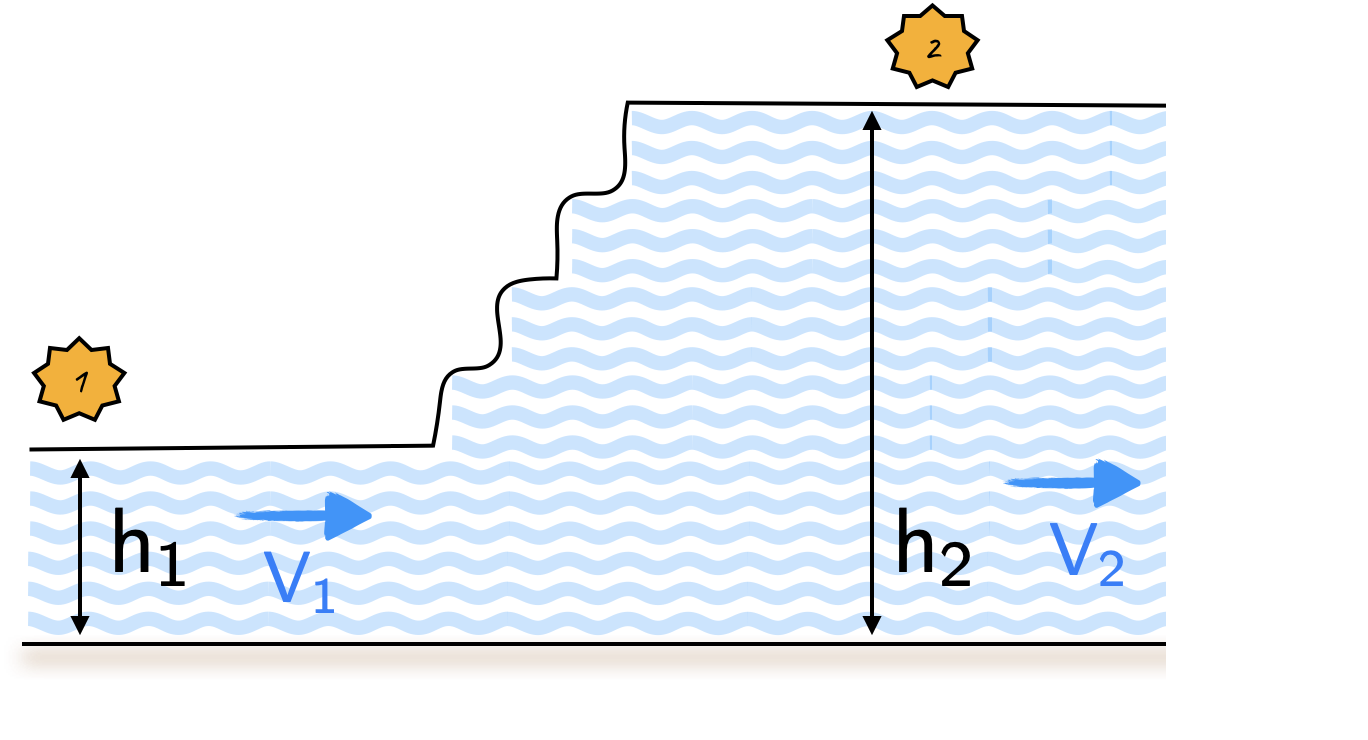
\includegraphics[width=0.2\textwidth]{images/image_1.png}
    \caption{Cyclic heat engine.}
    \label{fig:enter-label}
\end{figure}

\begin{enumerate}
\item[a.] What assumption must one make on this cyclic heat engine to ensure that maximum possible work can be produced? ${\color[rgb]{0.028509,0.250925,0.501969}[2]}$
\vspace{1 cm}
\item[b.] Calculate the maximum possible work output that can be produced by the device.  ${\color[rgb]{0.028509,0.250925,0.501969}[8]}$
\\
\vspace{8 cm}
\end{enumerate}

\hfill\break

\vspace{4 cm}

\hypertarget{problem-4}{%
\subsection{Problem 4}\label{problem-4}}

Please clarify whether the entire statement is true or false. You are
\textbf{not} required to justify your answers for statements.

\begin{enumerate}
\item[a.] Shock-induced boundary layer separation and viscous dissipation are examples of irreversibilities. ${\color[rgb]{0.028509,0.250925,0.501969}[1]}$

\item[b.] The entropy of a system is an extensive thermodynamic property. It represents the inability of a system's thermal energy to yield useful mechanical work. ${\color[rgb]{0.028509,0.250925,0.501969}[1]}$

\item[c.] For perfect gases, ${\color[rgb]{0.878548,0.880173,0.060757}c}_{\color[rgb]{0.079785,0.618358,0.483717}V}$ and ${\color[rgb]{0.986252,0.007236,0.027423}c}_{\color[rgb]{0.315209,0.728565,0.037706}p}$ are not constant. ${\color[rgb]{0.028509,0.250925,0.501969}[1]}$

\item[d.] Enthalpy is by definition the sum of internal energy and pressure multiplied by volume, i.e., ${\color[rgb]{0.986252,0.007236,0.027423}H} = {\color[rgb]{0.878548,0.880173,0.060757}U} + {\color[rgb]{0.315209,0.728565,0.037706}p}{\color[rgb]{0.079785,0.618358,0.483717}V}$. ${\color[rgb]{0.028509,0.250925,0.501969}[1]}$

\item[e.] There are three main ways for heat to transfer: (i) conduction; (ii) radiation, and (iii) convection. ${\color[rgb]{0.028509,0.250925,0.501969}[1]}$

\item[f.] All adiabatic processes are reversible. ${\color[rgb]{0.028509,0.250925,0.501969}[1]}$

\item[g.] Isentropic compression can be shown as a vertically straight line between two isobars on a temperature vs. specific entropy graph, i.e., ${\color[rgb]{0.164799,0.878862,0.723179}T}$ vs. ${\color[rgb]{0.599997,0.600015,0.600005}s}$. The higher pressure values lie vertically above lower pressure values. ${\color[rgb]{0.028509,0.250925,0.501969}[1]}$

\end{enumerate}



\end{document}
